% Autor: Kamil Ziemian

% ---------------------------------------------------------------------
% Podstawowe ustawienia i pakiety
% ---------------------------------------------------------------------
\RequirePackage[l2tabu, orthodox]{nag}  % Wykrywa przestarzałe i niewłaściwe
% sposoby używania LaTeXa. Więcej jest w l2tabu English version.
\documentclass[a4paper,11pt]{article}
% {rozmiar papieru, rozmiar fontu}[klasa dokumentu]
\usepackage[MeX]{polski}  % Polonizacja LaTeXa, bez niej będzie pracował
% w języku angielskim.
\usepackage[utf8]{inputenc} % Włączenie kodowania UTF-8, co daje dostęp
% do polskich znaków.
\usepackage{lmodern}  % Wprowadza fonty Latin Modern.
\usepackage[T1]{fontenc}  % Potrzebne do używania fontów Latin Modern.



% ------------------------------
% Podstawowe pakiety (niezwiązane z ustawieniami języka)
% ------------------------------
\usepackage{microtype}  % Twierdzi, że poprawi rozmiar odstępów w tekście.
% \usepackage{graphicx}  % Wprowadza bardzo potrzebne komendy do wstawiania
% grafiki.
\usepackage{vmargin}  % Pozwala na prostą kontrolę rozmiaru marginesów,
% za pomocą komend poniżej. Rozmiar odstępów jest mierzony w calach.
% ------------------------------
% MARGINS
% ------------------------------
\setmarginsrb
{ 0.7in} % left margin
{ 0.6in} % top margin
{ 0.7in} % right margin
{ 0.8in} % bottom margin
{  20pt} % head height
{0.25in} % head sep
{   9pt} % foot height
{ 0.3in} % foot sep



% ------------------------------
% Często używane pakiety
% ------------------------------
% \usepackage{csquotes}  % Pozwala w prosty sposób wstawiać cytaty do tekstu.
% \usepackage{xcolor}  % Pozwala używać kolorowych czcionek (zapewne dużo
% więcej, ale ja nie potrafię nic o tym powiedzieć).



% ------------------------------
% Pakiety do tekstów z nauk przyrodniczych
% ------------------------------
\let\lll\undefined  % Amsmath gryzie się z pakietami do języka
% polskiego, bo oba definiują komendę \lll. Aby rozwiązać ten problem
% oddefiniowuję tę komendę, ale może tym samym pozbywam się dużego Ł.
\usepackage[intlimits]{amsmath}  % Podstawowe wsparcie od American
% Mathematical Society (w skrócie AMS)
\usepackage{amsfonts, amssymb, amscd, amsthm}  % Dalsze wsparcie od AMS
\usepackage{upgreek}  % Ładniejsze greckie litery
% Przykładowa składnia: pi = \uppi
\usepackage{calrsfs}  % Zmienia czcionkę kaligraficzną w \mathcal
% na ładniejszą. Może w innych miejscach robi to samo, ale o tym nic
% nie wiem.



% ---------------
% Wspaniały pakiet PGF/TikZ
% ---------------
\usepackage{tikz}

\usetikzlibrary{decorations.markings}  % Włączenie konkretnych bibliotek
% pakietu TikZ



% ---------------
% Tworzenie otoczeń "Twierdzenie", "Definicja", "Lemat", etc.
% ---------------
\newtheorem{twr}{Twierdzenie}  % Komenda wprowadzająca otoczenie
% ,,twr'' do pisania twierdzeń matematycznych
\newtheorem{defin}{Definicja}  % Analogicznie jak powyżej
\newtheorem{wni}{Wniosek}



% ------------------------------
% Pakiety których pliki *.sty mają być w tym samym katalogu co ten plik
% ------------------------------
\usepackage{mathcommands}
\usepackage{latexshortcuts}
\usepackage{calculuscommands}




% ---------------------------------------------------------------------
% Dodatkowe ustawienia dla języka polskiego
% ---------------------------------------------------------------------
\renewcommand{\thesection}{\arabic{section}.}
% Kropki po numerach rozdziału (polski zwyczaj topograficzny)
\renewcommand{\thesubsection}{\thesection\arabic{subsection}}
% Brak kropki po numerach podrozdziału



% ------------------------------
% Ustawienia różnych parametrów tekstu
% ------------------------------
\renewcommand{\arraystretch}{1.2}  % Ustawienie szerokości odstępów między
% wierszami w tabelach



% ------------------------------
% Pakiet „hyperref”
% Polecano by umieszczać go na końcu preambuły
% ------------------------------
\usepackage{hyperref}  % Pozwala tworzyć hiperlinki i zamienia odwołania
% do bibliografii na hiperlinki










% --------------------------------------------------------------------
% Tytuł, autor, data
\title{Analiza matematyczna --~błędy i~uwagi}

% \author{}
% \date{}
% --------------------------------------------------------------------










% ####################################################################
\begin{document}
% ####################################################################





% ######################################
\maketitle  % Tytuł całego tekstu
% ######################################





% ######################################
% \newpage
\section{Analiza zespolona}

\vspace{\spaceTwo}
% ######################################



% ############################
\Work{ % Autor i tytuł dzieła
  Franciszek Leja \\
  „Funkcje zespolone”, \cite{LejaFunkcjeZespolone2006} }
% Sprawdź tu wszystkie eqref.


\CenterBoldFont{Uwagi}

\start W~książce często mówi~się o~prostej na~płaszczyźnie
zespolonej~$\Cbb$, jednak prawie zawsze chodzi o~prostą w~sensie
płaszczyzny rzeczywistej $\Cbb \simeq \Rbb^{ 2 }$. W~dodatku \textit{Wstęp
  do~teorii funkcji analitycznych wielu zmiennych} Józefa Siciaka
wprowadza~się pojęcie prostej zespolonej, która w~przypadku
płaszczyzny zespolonej~$\Cbb$ jest po prostu jej równa.

\vspace{\spaceFour}



\start W~analizie zespolonej jest praktycznie użyteczne wprowadzenie
zwięzłego oznaczenie na~otoczenie pierścieniowe
\begin{equation}
  \label{eq:Leja-01}
  \Pier(a, r, R) := \{ z \;|\; r < \absOne{ z - a } < R \}.
\end{equation}

\vspace{\spaceFour}



\start \Str{7} Powinna już tu być podana podstawowa własność jednostki
urojonej~$i^{ 2 } = -1$, nie zaś dopiero na~stronie 9. Bez~tego, bądź
jakiegoś innego wyjaśnienia, ciężko zrozumieć czym tak naprawdę~są
liczby postaci $\alpha + \beta i$.

\vspace{\spaceFour}



\start \Str{8--9} Aby~wyrażenie $1 / z = \zbar / ( z \zbar )$ miało
sens, należy chyba postępować w~następujący sposób\footnote{Leja
  zapewne zdawał sobie z~tego sprawę, jednak według mnie nie~zaznaczył
  tego wystarczająco jasno w~tekście.}. Na~początku należy zdefiniować
mnożenie liczb zespolonych, z~tego zaś wynika wzór na dzielenie liczb
zespolonych przez liczbę rzeczywistą~$a \neq 0$
\begin{equation}
  \label{eq:Leja-02}
    \frac{ z }{ a } = \frac{ 1 }{ a } \cdot z.
\end{equation}
Z~niemożliwości obliczenia $1 / 0$ w~liczba rzeczywistych wynika więc
niemożliwość zrobienia tego samego w~liczbach zespolonych. Ponieważ
odwrotność liczby jest liczbą rzeczywistą daną wzorem
\begin{equation}
  \label{eq:Leja-03}
  \frac{ 1 }{ a + i0 } = \frac{ 1 }{ a } + i0
  = \frac{ 1 }{ a },
\end{equation}
więc dzielenie liczby zespolonej przez rzeczywistą wynika teraz z~ich
reguł mnożenia. Teraz możemy \textit{zdefiniować} dla~$z \neq 0$ liczbę
$1 / z$ wzorem
\begin{equation}
  \label{eq:Leja-04}
    \frac{ 1 }{ z } := \frac{ \zbar }{ z \zbar }.
\end{equation}
Ponieważ $z \zbar$ jest liczbą rzeczywistą, więc dzielenie przez nią
wynika z~pojęć już wprowadzonych. Gdy $z = 0$ wtedy $z \zbar = 0$,
widzimy więc, że~również w~przypadku liczb zespolonych nie jest
możliwe dzielenie przez~0.

Teraz należy sprawdzić, czy tak wprowadzone dzielenie przez liczbę
zespoloną posiada te same własności, co dzielenie liczb rzeczywistych.
Na~przykład, że~zachodzi
\begin{equation}
  \label{eq:Leja-05}
    ( 1 / z ) / w = 1 / ( z w ), \quad z, w \in \Cbb.
\end{equation}
Tą tożsamość można udowodnić w~następujący sposób
\begin{equation}
  \label{eq:Leja-06}
  \begin{split}
    ( 1 / z ) / w =
    \left( \frac{ \zbar }{ z \zbar } \right) / w
    = \frac{ \zbar }{ z \zbar } \frac{ \wbar }{ w \wbar }
    = \frac{ 1 }{ z \zbar } \frac{ 1 }{ w \wbar } ( \zbar \wbar )
    = \frac{ 1 }{ z \zbar w \wbar } ( \zbar \wbar )
    = \frac{ 1 }{ z w \zbar \wbar } ( \zbar \wbar )
    = 1 / ( z w ).
  \end{split}
\end{equation}

\vspace{\spaceFour}



\start \Str{9--10} Według wszystkich mi znanych historycznych prac na
temat liczb zespolonych, zostały one odkryte już w~XVI wieku podczas
badania rozwiązań równania \textit{trzeciego} stopnia, nie zaś równań
kwadratowych. \red{Zacytuj tu jakąś dobrą pozycję historyczną.}

\vspace{\spaceFour}



\start \Str{10} Przy określaniu argumentu liczby zespolonej pierwszy
raz pojawia~się problem często spotykany w~analizie zespolonej
mianowicie, że~wielu funkcji nie da~się określić jako zwykłych funkcji
liczbowych, które liczbie zespolonej przyporządkowują liczbę
zespoloną. Sam zapis wyrażenia $\arg z$ sugeruje, że~argument jest
zwykłą funkcją liczbową zmiennej~$z$, jednak
z~definicji\footnote{Niezależnie którą~się przyjmuje.} wynika,
że~istnieje jednak nieskończenie wiele liczb odpowiadających
zapisowi\footnote{Dla liczy~$0$ można uznać
  dowolną liczbę rzeczywistą za~jej argument, ale~to pojęcie nie jest
  użyteczne, więc nie będziemy~się nim zajmować.}~$\arg z$, przy $z \neq 0$. Są~one postaci
\begin{equation}
  \label{eq:Leja-07}
  \arg z = \Arg z + 2\pi k, \quad k = 0, \pm 1, \pm 2, \ldots,
\end{equation}
gdzie $\Arg z$ jest już zwyczajną funkcją liczbową.
Wyrażenie~$\arg z$, przy ustalonym~$z$, oznacza więc nie liczbę lecz
przeliczalny zbiór liczb. Jest to przykład jednego z~typów funkcji
wielowartościowych.

Właściwym sposobem rozwiązania zagadnienia tego typu
funkcji\footnote{A~przynajmniej najlepszym obecnie znanym.} jest
rozważanie $\arg z$, przy $z \neq 0$, jako funkcji nie na~płaszczyźnie
zespolonej, lecz na~odpowiedniej powierzchni Riemanna. Ponieważ jednak
jest to już dość zaawansowana część analizy zespolonej, tutaj
ograniczymy~się do~omówienia, dlaczego najprostszy sposób rozwiązania
tego nie jest wystarczający.

Rozwiązanie to~polega na~ograniczeniu~się do~argumentów
zawierających~się w~przedziale $( -\pi, \pi ]$. Jednak już na~poziomie
wyprowadzenia wzoru na~pierwiastek $n$-tego stopnia (str.~11--12)
staje~się to~nieprzyjemnie ograniczające. Oprócz tego, funkcja ta nie
byłaby ciągła na~os $\arg z = \pi$, co~w~dalszym ciągu okaże~się
bardzo niewygodnie (pierwsze znaki tego znaleźć można na~stronach
59--60).

\vspace{\spaceFour}



\start \Str{12} Należy silniej niż w~tekście podkreślić,
że~$\sqrt[n]{ z }$ nie jest zwykłą funkcją liczbową, lecz~funkcją
$n$-wartościową, nie można więc jej używać w~ten sam sposób co~funkcji
jednowartościowych\footnote{Pisał już o~tym Frege, zobacz część
  poświęcona jego filozofii w~G. E. M. Anscombe P. T. Geach,
  \textit{Trzej filozofowie} \cite{AnscombeGeachTrzejFilozofowie1981}.}.
Zapomnienie o~tym prowadzi do~znanego paradoksu. Mamy mianowicie
\begin{equation}
  \label{eq:Leja-08}
  -1 = i \cdot i = \sqrt{ -1 } \cdot \sqrt{ -1 } = \sqrt{ ( -1 ) \cdot ( -1 ) }
  = \sqrt{ 1 } = 1.
\end{equation}

Pojawiają~się tu dwa błędy, mające to~samo źródło. Po~pierwsze
$\sqrt{ -1 } = \{ i, -i \}$ więc w~równaniu powyżej mamy mnożenie
nie liczb zespolonych, lecz zbiorów liczb zespolonych, więc to co~się
naprawdę dzieje w~powyższym wzorze przestaje być oczywisty. W~istocie
zauważmy, że~wynik powyższych obliczeń można otrzymać w~następujący
sposób
\begin{equation}
  \label{eq:Leja-09}
  ( -i ) \cdot i = 1.
\end{equation}
Drugi błąd jest następując. Jeśli rozważamy~$1$ jako liczbę zespoloną,
to
\begin{equation}
  \label{eq:Leja-10}
  \sqrt{ 1 } = \{ 1, -1 \},
\end{equation}
czyli otrzymany poprzednio wynik $\sqrt{ 1 }$~„$=$”~$1$, przedstawia
tylko jeden element zbioru $\sqrt{ 1 }$.

Wymaga to~pewnego komentarza. Jeśli będziemy rozpatrywać operację
pierwiastkowania na~zbiorze $D = \{ x \, | \, x \geq 0 \}$, to jest
możliwe zdefiniowanie na~nim funkcji
$\sqrt{ \cdot }: x \mapsto \sqrt{ x }$, która jest zwykłą funkcją
liczbową, jednowartościową. Kiedy jednak rozpatrujemy liczby
zespolone~$\Cbb$, wówczas takiej funkcji jednowartościowej nie~da~się
określić na~całej płaszczyźnie zespolonej. Jeśli więc pierwiastkujemy
$-1$, co musimy robić w~zbiorze liczb zespolonych, to~popełniamy
niespójność w~rozumowaniu, gdy~pierwiastkując~$1$ nagle ograniczamy
nasze rozumowanie tylko do~zbioru liczb rzeczywistych,
nieujemnych~$D$.

Warto zwrócić uwagę, że~jednoznaczną funkcję
$\sqrt[ n ]{ \cdot }: z \mapsto \sqrt[ n ]{ z }$ na~pewnych właściwych
podzbiorach $\Cbb$. Wynika to~między innymi z~twierdzenia o~istnieniu
jednoznacznych gałęzi logarytmu, zobacz str.~95 w~komentowanej
tu~książce \cite{LejaFunkcjeZespolone2006}. Tym problemem nie
będziemy~się w~tym miejscu szerzej zajmować.

\vspace{\spaceFour}



\start \Str{12--13} W~przeprowadzonych tu rachunkach, trzeba w~pewnym
momencie skorzystać z~tego, że~równanie $x^{ 2 } = \alpha$,
$\alpha > 0$ ma tylko dwa rozwiązania rzeczywiste
$\pm \sqrt{ \alpha }$. Wynika to~ze~wzoru~(9), ale~zamysł tych
obliczeń polega na~tym, by~z~niego nie korzystać. W~tym momencie nie
wiem, jak należałoby to~poprawić.

\vspace{\spaceFour}



\start \Str{13} Paragraf o~obliczaniu $\sqrt{ \alpha + i \beta }$
kieruje~się chyba następującą myślą. Aby znaleźć te pierwiastki musimy
obliczyć funkcje trygonometryczne dla~$\theta_{ 0 } = \varphi / 2$,
$\theta_{ 1 } = \varphi / 2 + \pi$. Można łatwo wyrazić $\cos \varphi$
i~$\sin \varphi$ za~pomocą $\alpha$ i~$\beta$. Teraz możemy obliczyć
\begin{equation}
  \label{eq:Leja-11}
    \cos \theta_{ 0 } = \cos \tfrac{ \varphi }{ 2 } = \frac{ 1 }{ 2 } ( 1 + \cos \varphi ),
\end{equation}
podobnie dla~funkcji $\sin$. Drugi pierwiastek obliczamy za~pomocą
wzorów
\begin{equation}
  \label{eq:Leja-12}
  \cos( \tfrac{ \varphi }{ 2 } + \pi ) = -\cos( \tfrac{ \varphi }{ 2 } ), \quad
  \sin( \tfrac{ \varphi }{ 2 } + \pi ) = -\sin( \tfrac{ \varphi }{ 2 } ).
\end{equation}
Tym samym możemy wyrazić oba szukane pierwiastki w~prosty sposób
za~pomocą $\alpha$ i~$\beta$.

\vspace{\spaceFour}



\start \Str{20} Warto byłoby przytoczyć skąd~się bierze wzór na
iloczyn Cauchy’ego szeregów. Gdybyśmy wzięli dwa szeregi potęgowe
i~mnożyli je tak jakby były zwykłymi wielomianami, wówczas
\begin{equation}
  \label{eq:Leja-13}
    \left( \sum_{ n = 0 }^{ \infty } a_{ n } z^{ n } \right) \left(
      \sum_{ m = 0 }^{ \infty } b_{ m } z^{ m } \right) = \sum_{ n = 0
    }^{ \infty } ( a_{ n } b_{ 0 } + a_{ n - 1 } b_{ 1 } + \ldots + a_{ 0
    } b_{ n } ) z^{ n }.
\end{equation}
Należy jednak pamiętać, że~rachunki te są nieścisłe i~mogą być
matematycznie niepoprawne dla~pewnych szeregów potęgowych. Dostarczają
jednak uzasadnienia dla tego sposobu mnożenia szeregów.

\vspace{\spaceFour}



\start \Str{20} Zauważmy, że~w~twierdzeniu udowodnionym przez
Mertensa, wystarczy wykazać zbieżność iloczynu szeregów, bowiem
wartość tej granicy wynika z~twierdzenia Abela.

\vspace{\spaceFour}



\start \Str{20--21} Dowód twierdzenia Mertensa jest według mnie
przeprowadzony zbyt szybko, dlatego tutaj postaramy~się go uzupełnić
w~kilku miejscach.

Chcemy pokazać, że~dla wszystkich $n > N$, przy pewnym skończonym~$N$,
zachodzi poniższa nierówność
\begin{equation}
  \label{eq:Leja-14}
    \absOne{ C_{ n } - A_{ n } B } \leq \varepsilon, \quad \forall \varepsilon > 0,
\end{equation}
bowiem z~tego będzie wynikać
\begin{equation}
  \label{eq:Leja-15}
  \absOne{ C_{ n } - AB }
  \leq \absOne{ C_{ n } - A_{ n } B } + \absOne{ A_{ n } B - AB } \leq 2 \varepsilon,
\end{equation}
dla wszystkich $n > N_{ 1 }$. Ustalmy najpierw $\varepsilon > 0$. Teraz
dobierzmy takie $p$, że~dla $n > p$ zachodzi nierówność
$\absOne{ \beta_{ n } } < \varepsilon / 2K$. Teraz zachodzi nierówność
\begin{equation}
  \label{eq:Leja-16}
  \begin{split}
    \absOne{ C_{ n } - A_{ n } B }
    &=
      \absOne{ a_{ 0 } \beta_{ n } + a_{ 1 } \beta_{ n - 1 } + \ldots + a_{ n } \beta_{ 0 } }
      \leq
      \absOne{ a_{ 0 } } \absOne{ \beta_{ n } }
      + \absOne{ a_{ 1 } } \absOne{ \beta_{ n - 1 } } + \ldots
      + \absOne{ a_{ n - p + 1 } } \absOne{ \beta_{ p + 1 } } \, + \\
    &\hspace{1.5em} + \absOne{ a_{ n - p } \beta_{ p } + \ldots + a_{ n } \beta_{ 0 } }
      \leq
      \frac{ \varepsilon }{ 2K }
      ( \absOne{ a_{ 0 } } + \ldots + \absOne{ a_{ n - p + 1 } } )
      + \absOne{ a_{ n - p } \beta_{ p } + \ldots + a_{ n } \beta_{ 0 } }.
  \end{split}
\end{equation}
Pierwszy wyraz jest $\leq \epsilon / 2$. Dla drugiego wyrazu mamy
\begin{equation}
  \label{eq:Leja-17}
  \absOne{ a_{ n - p } \beta_{ p } + \ldots + a_{ n } \beta_{ 0 } }
  \leq
  \absOne{ a_{ n - p } } \absOne{ \beta_{ p } } + \ldots + \absOne{ a_{ n } }
  \absOne{ \beta_{ 0 } }
  \leq M_{ p } ( \absOne{ a_{ n - p } } + \ldots + \absOne{ a_{ n } } ),
\end{equation}
gdzie
$M_{ p } = \max( \absOne{ \beta_{ 1 } }, \ldots, \absOne{ \beta_{ p } } )$.
Ponieważ~$p$ jest ustalone możemy dobrać takie $q$, że~dla każdego
$n > q$ zachodzić $\absOne{ a_{ n - p } } < \varepsilon / ( 2 p M_{ p } )$.
Teraz dla każdego $n > \max( p, q )$ zachodzi
\begin{equation}
  \label{eq:Leja-18}
  \absOne{ C_{ n } - AB } \leq \varepsilon.
\end{equation}
Możemy więc przyjąć $N = \max( p, q )$ i~tym samym dowód jest
zakończony.

\vspace{\spaceFour}



\start \Str{22} Dowód twierdzenia Abela nie jest wcale oczywisty,
dlatego tu~postaram się go uzupełnić tu i~w~następny punkcie.
Po~pierwsze dowód formuły
\begin{equation}
  \label{eq:Leja-19}
  \frac{ C_{ 0 } + C_{ 1 } + \ldots + C_{ n - 1 } }{ n }
  = AB + A q_{ n } + B p_{ n } + r_{ n },
\end{equation}
nie jest taki oczywista. Pokażemy tu, że~zachodzi równoważna formuła
\begin{equation}
  \label{eq:Leja-20}
  C_{ 0 } + C_{ 1 } + \ldots + C_{ n - 1 }
  = n AB + A ( \beta_{ 0 } + \beta_{ 1 } + \ldots + \beta_{ n - 1 } )
  + B ( \alpha_{ 0 } + \alpha_{ 1 } + \ldots + \alpha_{ n - 1 } ) + R_{ n },
\end{equation}
gdzie
\begin{equation}
  \label{eq:Leja-21}
  R_{ n } = n r_{ n } =
  \alpha_{ n - 1 } \beta_{ 0 } + \alpha_{ n - 2 } \beta_{ 1 } + \ldots + \alpha_{ 0 } \beta_{ n - 1 }.
\end{equation}
Łatwo~się o~jej prawdziwości przekonać, wypisując kilka pierwszych
wyrazów.

Musimy jednak najpierw wykazać wynik pomocniczy:
\begin{equation}
  \label{eq:Leja-22}
  \begin{split}
    \sum_{ i = 0 }^{ n } c_{ i } = \sum_{ i = 0 }^{ n } ( a_{ i } b_{
      0 } + a_{ i - 1 } b_{ 1 } + \ldots + a_{ 0 } b_{ i } ) &= ( a_{ 0 }
    + a_{ 1 } + \ldots + a_{ n } ) b_{ 0 } + ( a_{ 0 } + a_{ 1 }
    + \ldots + a_{ n - 1 } ) b_{ 1 } \, + \\
    &\hspace{1.5em} + \ldots + a_{ 0 } b_{ n }.
  \end{split}
\end{equation}
Wzór ten jest dość oczywisty, jeśli~się prześledzi kilka pierwszych
przypadków. Dowód przeprowadzimy indukcyjnie. Przypadek $n = 0$
wychodzi sam, zakładają, że~dla $n$ wynik jest już wykazany obliczmy
\begin{equation}
  \label{eq:Leja-23}
  \begin{split}
    \sum_{ i = 0 }^{ n + 1 } c_{ i }
    &= ( a_{ 0 } + a_{ 1 } + \ldots +
    a_{ n } ) b_{ 0 } + ( a_{ 0 } + a_{ 1 } + \ldots + a_{ n - 1 } ) b_{
      1 } + \ldots + a_{ 0 } b_{ n } + c_{ n + 1 } \, + \\
    &= ( a_{ 0 } + a_{ 1 } + \ldots + a_{ n } ) b_{ 0 } + ( a_{ 0 } + a_{
      1 }
    + \ldots + a_{ n - 1 } ) b_{ 1 } + \ldots + a_{ 0 } b_{ n } \, + \\
    &\hspace{1.5em}
      + a_{ n + 1 } b_{ 0 } + a_{ n } b_{ 1 } + \ldots + a_{ 0 } b_{ n + 1
    }
    = ( a_{ 0 } + a_{ 1 } + \ldots + a_{ n } + a_{ n + 1 } ) b_{ 0 } \, + \\
    &\hspace{1.5em} + ( a_{ 0 } + a_{ 1 } + \ldots + a_{ n - 1 } + a_{ n } ) b_{ 1 } +
    \ldots + ( a_{ 0 } + a_{ 1 } ) b_{ 0 } + a_{ 0 } b_{ n + 1 }.
  \end{split}
\end{equation}

Możemy teraz przejść do~dowodu wzoru \eqref{eq:Leja-16}, który również
przeprowadzimy indukcyjnie. Dla~$n = 0$ wynika to z~prostego rachunku.
Zadłużmy, że~jest to prawdą dla~$n$~i~udowodnijmy dla~$n + 1$.
\begin{equation}
  \label{eq:Leja-24}
  \begin{split}
    C_{ 0 } + C_{ 1 } + \ldots + C_{ n - 1 } + C_{ n }
    &= n AB + A \sum_{ i = 0 }^{ n - 1 } \beta_{ i } + B \sum_{ i = 0 }^{ n - 1 }
      \alpha_{ i } + R_{ n } + C_{ n }.
  \end{split}
\end{equation}
Następny krok jest trochę długi. Przeliczając kilka pierwszych
przypadków, łatwo zgadnąć, że
\begin{equation}
  \label{eq:Leja-25}
    C_{ n } = AB + A \beta_{ n } + B \alpha_{ n } - R_{ n } + R_{ n + 1 }.
\end{equation}
Zacznijmy od~tego, że
$b_{ n } = B_{ n } - B_{ n - 1 } = \beta_{ n } - \beta_{ n - 1 }$,
korzystając więc, ze~wzoru \eqref{eq:Leja-19}
\begin{equation}
  \label{eq:Leja-26}
  \begin{split}
    C_{ n }
    &= A_{ n } b_{ 0 } + A_{ n - 1 } b_{ 1 } + \ldots + A_{ 0 }
      b_{ n } = ( A + \alpha_{ n } ) ( B + \beta_{ 0 } ) + ( A + \alpha_{ n - 1 } )
      ( \beta_{ 1 } - \beta_{ 0 } ) \, + \\
    &\hspace{1.5em} + ( A + \alpha_{ n - 2 } )( \beta_{ 2 } - \beta_{ 1 } ) + \ldots
      + ( A + \alpha_{ 0 } ) ( \beta_{ n } - \beta_{ n - 1 } )
      = AB + B \alpha_{ n } + \alpha_{ n } \beta_{ 0 } \, + \\
    &\hspace{1.5em} + A \beta_{ 0 } + A ( \beta_{ 1 } - \beta_{ 0 } + \beta_{ 2 }
      - \beta_{ 1 } + \ldots + \beta_{ n } - \beta_{ n - 1 } ) + \alpha_{ n - 1 } ( \beta_{ 1 } - \beta_{ 0 } )
      + \alpha_{ n - 2 } ( \beta_{ 2 } - \beta_{ 1 } ) \, + \\
    &\hspace{1.5em} + \ldots + \alpha_{ 0 } ( \beta_{ n } - \beta_{ n - 1 } ) = \\
    &=
      AB + A \beta_{ n } + B \alpha_{ n } + \alpha_{ n } \beta_{ 0 } + \alpha_{ n - 1 } \beta_{ 1 }
      + \alpha_{ n - 2 } \beta_{ 2 } + \ldots + \alpha_{ 0 } \beta_{ n } - \\
    &\hspace{1.5em} - ( \alpha_{ n - 1 } \beta_{ 0 } + \alpha_{ n - 2 } \beta_{ 1 }
      + \ldots + \alpha_{ 0 } \beta_{ n - 1 } ) = \\
    &= AB + A \beta_{ n } + B \alpha_{ n } + R_{ n + 1 } - R_{ n }.
  \end{split}
\end{equation}
Warto pamiętać, że~suma $C_{ 0 } + C_{ 1 } + \ldots + C_{ n }$ odpowiada
liczbie~$n + 1$. Tym samym
\begin{equation}
  \label{eq:Leja-27}
  \begin{split}
    C_{ 0 } + C_{ 1 } + \ldots + C_{ n - 1 } + C_{ n }
    &= n AB + A \sum_{ i = 0 }^{ n - 1 } \beta_{ i } + B \sum_{ i = 0 }^{ n - 1 }
      \alpha_{ i } + R_{ n } + C_{ n } = \\
    &= ( n + 1 ) AB + A \sum_{ i = 0 }^{ n } \beta_{ i } + B \sum_{ i = 0 }^{ n } \alpha_{ i }
      + R_{ n + 1 }.
  \end{split}
\end{equation}

\vspace{\spaceFour}



\start \Str{22} Potrzebujemy jeszcze udowodnić,
że~$\lim_{ n \to \infty } r_{ n } = 0$. Ponieważ $\alpha_{ n }$
i~$\beta_{ n }$ są zbieżne istnieją więc stałe $M_{ \alpha }$
i~$M_{ \beta }$ takie, że
\begin{equation}
  \label{eq:Leja-28}
    \absOne{ M_{ \alpha } } \leq M_{ \alpha }, \quad \absOne{ \beta_{ n } } \leq M_{ \beta }.
\end{equation}
Ustalmy teraz $\varepsilon > 0$. Skoro $\beta_{ n }$ jest zbieżny do~0,
więc możemy znaleźć taką liczbę~$p$,
iż~$\absOne{ \beta_{ n } } \leq \varepsilon / 2 M_{ \alpha }$, dla~$n > p$.
Teraz
\begin{equation}
  \label{eq:Leja-29}
  \begin{split}
    \absOne{ r_{ n } }
    &=
      \frac{ 1 }{ n } \absOne{ \alpha_{ n - 1 } \beta_{ 0 } + \alpha_{ n - 2 } \beta_{ 1 }
      + \ldots + \alpha_{ n - p - 1 } \beta_{ p } + \ldots + \alpha_{ 0 } \beta_{ n - 1 } } \leq \\
    &\leq \frac{ 1 }{ n } \absOne{ \alpha_{ n - 1 } \beta_{ 0 } + \alpha_{ n - 2 } \beta_{ 1 }
      + \ldots + \alpha_{ n - p - 1 } \beta_{ p } } + \frac{ 1 }{ n }
    \absOne{ \alpha_{ n - p - 2 } \beta_{ p + 1 } + \ldots + \alpha_{ 0 } \beta_{ n - 1 } } \leq \\
    &\leq \frac{ p + 1 }{ n } M_{ \alpha } M_{ \beta }
      + \frac{ n - p - 1 }{ n } M_{ \alpha } \frac{ \epsilon }{ 2 M_{ \alpha } }
      = \frac{ p + 1 }{ n } M_{ \alpha } M_{ \beta } + \frac{ n - p - 1 }{ n }
    \frac{ \varepsilon }{ 2 } \leq \\
    &\leq \frac{ \varepsilon }{ 2 } + \frac{ p + 1 }{ n } M_{ \alpha } M_{ \beta }.
  \end{split}
\end{equation}
Ponieważ $p$~jest ustalone, więc istnieje takie~$q$, że~dla $n > q$
drugi człon jest również mniejszy od~$\varepsilon / 2$, co~kończy dowód.

\vspace{\spaceFour}



\start \Str{25} Wedle definicji zbiór pusty jest domknięty, jednak
przy omawianiu własności przecięć zbiorów domkniętych, jest tu
wymieniony osobno.

\vspace{\spaceFour}



\start \Str{28--29} Jest to przykład bałaganu pojęciowego
najczystszego rodzaju. Najpierw na~stronie~28 definiuje~się krzywą
jako zbiór punktów, by na~stronie następnej stronie zwraca~się uwagę,
że~należy odróżnić krzywą od~jej zbioru punktów.

Problem wynika z~pierwszej definicji, wedle której krzywa to~zbiór
punktów dany przez odpowiednią funkcje. Aby~rozwiązać ten problem,
należy zdefiniować krzywą jako funkcję zespoloną~$z( t )$, ciągłą
na~pewnym przedziale~$I$ i~różną od~stałej. Wówczas wzór~(1)
na~stronie~28 przedstawia zbiór punktów tej krzywej.

Ponadto Leja wydaje~się używać pojęcia krzywej zarówno
dla~odwzorowania, jak i~dla jego obrazu, która interpretacja jest
właściwa wynika zwykle jasno z~kontekstu. Nie będziemy~się starali
doprecyzować jego słów w~każdej z~tych sytuacji, jednak warto~się
starać o~większą jasność i~precyzję tekstów matematycznych.

\vspace{\spaceFour}



\start \Str{29} Jeśli funkcja $\varphi( \tau )$ nie jest suriekcją
na~przedział~$I$, to wedle przyjętej definicji~$z( \varphi( \tau ) )$,
$\tau \in I_{ 1 }$ jest krzywą. Jedna w~tym wypadku jej zbiór punktów,
może być różny od~tej dla~krzywej~$z( t )$, $t \in I$, co~jednak nie
jest żadnym problemem dla~rozwijanej tu~teorii.

\vspace{\spaceFour}



\start \Str{30} Warto podkreślić wagę warunku $z'( t ) \neq 0$
w~definicji krzywej gładkiej. W~geometrii różniczkowej, krzywą o~tej
własności nazywa~się \textbf{regularną}. Jeśli rozważana krzywa nie
jest regularna, to może~się zdarzyć, że~funkcja~$s( t )$ nie jest
monotoniczne rosnąc, lecz tylko niemalejąca i~na przedziałach stała,
tym samym nieodwracalna i~stwierdzenie, iż~istnieje parametr
kanoniczny jest nieprawdziwe.

Powód tego jest dość oczywisty. Jeśli krzywa ma~\textbf{punkty
  osobliwe}, czyli punkty w~których~$z'( t ) = 0$, to~możliwa jest
sytuacja, iż~pomimo zmieniającego~się parametru, będzie ona „stała
w~miejscu”. Przykładem takie zachowania jest krzywa
\begin{equation}
  \label{eq:Leja-30}
  z( t ) =
  \begin{cases}
    t^{ 2 } + i 0, & t \leq 0, \\
    0 + i 0, & t > 0.
  \end{cases}
\end{equation}
Jest to krzywa klasy $\Ccal^{ \infty }( \Rbb, \Cbb )$ NIE JEST, która
dla~$t \geq 0$ stoi w~punkcie $z = 0 + i 0$. Jeśli wzór na jej
długość, dostaniemy oczywisty rezultat
\begin{equation}
  \label{eq:Leja-31}
  \begin{split}
    s( t ) = \int_{ 0 }^{ t } \absOne{ z'( u ) } \, du = \int_{ 0 }^{ t } 0 \,
    du = 0, \quad t \geq 0.
  \end{split}
\end{equation}
Widzimy więc, że~krzywej tej nie da~się sparametryzować za~pomocą
zmiennej~$s$, czyli jej długości.

Jednak sama obecność punktów osobliwych, nie oznacza, że~krzywej nie
da~się przedstawić w~postaci równania kanonicznego. Jest to wciąż
możliwe, jeśli tych punktów jest „odpowiednio mało”. Przykładem
takiej sytuacji jest krzywa
\begin{equation}
  \label{eq:Leja-32}
  z( t ) = t^{ 3 } + i 0, \quad t \in \Rbb.
\end{equation}

Z~tego względu rozróżnia~się \textbf{punkty osobliwe krzywej}
i~\textbf{punkty osobliwe parametryzacja}
\cite{GdowskiElementGeometriiRozniczkowejZZadaniami1999}. Punkt
$z( t_{ 0 } )$ jest punktem osobliwym parametryzacja krzywej $z( t )$,
$t \in I = [ a, b ]$\footnote{Przedział ten może też być otwarty,
  skończony bądź nieskończony.}, jeśli $z'( t_{ 0 } ) = 0$ i~istnieje
reparametryzacja $\varphi: I_{ 1 } \to I$ taka,
że~$t_{ 0 } = \varphi( \tau_{ 0 } )$
i~$\tfrac{ d }{ d \tau } z\big( \varphi( \tau ) \big)|_{ \tau = \tau_{
    0 } } \neq 0$. Widzimy więc, że~tu problemem nie jest z~krzywą,
lecz z~pewną możliwą dla niej parametryzacja. Przykład
\eqref{eq:Leja-32} powyżej jest właśnie tego typu. Jeśli użyjemy
do~niego funkcji reparametryzującej
\begin{equation}
  \label{eq:Leja-33}
  \varphi( \tau ) =
  \begin{cases}
    -\sqrt[3]{ \absOne{ \tau } }, & \tau \leq 0, \\
    \sqrt[3]{ \tau }, & \tau > 0,
  \end{cases}
\end{equation}
otrzymamy
\begin{equation}
  \label{eq:Leja-34}
  z\big( \varphi( \tau ) \big) = \tau, \quad \tau \in \Rbb.
\end{equation}
Natomiast w~przypadku \eqref{eq:Leja-30} mamy do~czynienia z~punktami
osobliwymi krzywej, co~nie powinno nas dziwić. Problem polega tu
bowiem nie na~szczególnym wyborze parametryzacji, lecz na~tym,
że~krzywa od pewnego momentu stoi w~miejscu.

\vspace{\spaceFour}



\start \Str{30--31} Definicja krzywej przedziałami gładkiej jest
niepełna, skutkiem czego pojęcie wierzchołka takiej krzywej jest
błędne. Weźmy krzywą gładką na przedziale $[ \alpha, \beta ]$
i~podzielmy go dowolną ilością punktów w~dowolnych miejscach
na~podprzedziały, co jest zgodne z~przyjętą definicją. Tym samym
widzimy, że~krzywa ta składa~się z~dowolnej ilości łuków i~każdy punkt
jej obrazu jest jej wierzchołkiem. To~samo stosuje~się do krzywej
która jest nieróżniczkowalna w~punktach
$t_{ 1 }, t_{ 2 }, \ldots, t_{ p - 1 }$.

Rozwiązanie tego problemu jest proste, należy przyjąć, że~każdy z~tych
przedziałów był maksymalny w~następującym sensie. Jeśli krzywa
$z( t )$ jest gładka w~przedziale $[ t_{ k - 1 }, t_{ k } ]$, to nie
jest ona gładka w~przedziałach $[ t_{ k - 1 } - \epsilon, t_{ k } ]$
i~$[ t_{ k - 1 }, t_{ k } + \epsilon ]$ dla wszystkich~$\epsilon > 0$.

\vspace{\spaceFour}



\start \Str{32} Podana tu definicji krzywej zorientowanej dodatnio
jest z~praktycznego punktu widzenie
wystarczająca\footnote{Ja~przynajmniej nie znam przypadku, w~którym
  byłby problem z~określeniem czy~kontur jest dodatnio zorientowany
  czy też nie.}, jednak nieścisła. Wystarczy zadać pytanie, czy
idziemy po~krzywej „głową do~góry”, czy~„głową do~dołu”?

Przedstawione pojęcie orientacji krzywej intuicyjnie powinno działać
dla każdej krzywej, niezależnie od~tego czy jest gładka czy tylko
ciągła (w~tej zresztą ogólnej formie pojęcie orientacji jest
tu~podane). W~pełni ścisłe sformułowanie tego problemu nie jest wcale
łatwe. W~tej chwili najbardziej obiecujące wydaje mi~się podejście
w~którym najpierw definiuje~się orientację okręgu jednostkowego,
później zaś „homotopie zachowujące orientację”, za~krzywą
zorientowaną dodatnio uznać taką, która jest „homotopijna
z~zachowaniem orientacji z~okręgiem zorientowanym dodatnio”. O~ile
jednak zdefiniowanie okręgu zorientowanego dodatnio nie jest trudne,
to~podanie w~sposób ścisły i~wystarczająco ogólnych takich homotopii
przekracza moją wiedzę i~zdolności.

Dla zupełności zdefiniujemy tutaj \textbf{dodatnio zorientowany okrąg
  jednostkowy}. Definicja najkrótsza polega na~wskazaniu, że~okrąg ten
jest dany przez parametryzację $z( t ) = e^{ i t }$. Można podać
bardziej satysfakcjonujące definicje, bo~głębiej uzasadniające czemu
ta parametryzacja jest dodatnia, lecz biorąc pod uwagę, że~nie udało
mi~się zdefiniować odpowiednich homotopii i~tym samym główny problem
jest wciąż nie rozwiązany, nie ma to wielkiego sensu.

\vspace{\spaceFour}





% ##################
\begin{figure}

  \centering

  \label{fig:Leja-01}

  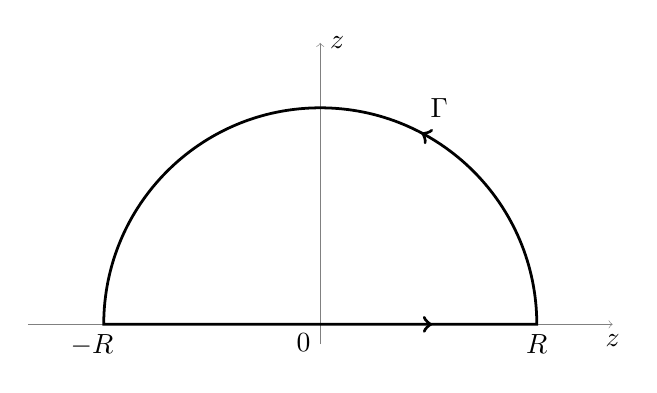
\begin{tikzpicture}
    \def\radius{2.75}

    \draw[help lines, ->] (-1.35 * \radius,0) -- (1.35 * \radius,0);

    \draw[help lines, ->] (0,-0.25) -- (0,1.3 * \radius);

    \draw [line width = 1pt, decoration = { markings, mark = at
      position 0.295 with {\arrow[line width=1.2pt]{>}}, mark = at
      position 0.6 with {\arrow[line width=1.2pt]{>}},}, postaction =
    {decorate} ] (-\radius, 0) -- (\radius, 0) arc (0:180:\radius) --
    cycle;


    \node at (1.35 * \radius,0) [below] {$\Real z$};

    \node at (0,1.3 * \radius) [right] {$\Imag z$};


    \node at (0,0) [below left] {$0$};

    \node at (-\radius - 0.15,0) [below] {$-R$};

    \node at (\radius,0) [below] {$R$};

    \node at (0.55 * \radius,2.75) {$\Gamma$};

  \end{tikzpicture}

  \caption{Jeden z~podstawowych konturów całkowania~$\Gamma$.}

\end{figure}
% ##################





\start \Str{32} Ze~względów praktycznych lepiej jest przyjąć,
że~kontur jest kawałkami gładką, a~nie po~prostu gładką, zorientowaną
dodatnio krzywą Jordana. W~praktyce bowiem do~najczęściej używanych
konturów są takie, które są tylko kawałkami gładkie, przykładem niech
będzie kontur~$\Gamma$ z~rysunku~(\ref{fig:Leja-01}).

W~tej chwili nie umiem rozstrzygnąć, czy~istnieje gładkie odwzorowanie
takie, że~jego obraz pokrywa~się z~kształtem~$\Gamma$ na~płaszczyźnie
zespolonej. Jednak nie jest to ważne, bowiem wykonując całkowanie
używa~się standardowo parametryzacji $\Gamma$, która gładka nie jest
(liniowej na~osi rzeczywistej, trygonometrycznej na~okręgu) i~nie
ma~żadnej praktycznej potrzeby by~taką była.

Należy zauważyć, że~pojęcie konturu używa~się w~praktyce nawet
w~ogólniejszych przypadkach, kiedy rozpatrywane krzywe mają punkty
wielokrotne. Takie jednak poszerzenie pojęcia konturu, odeszłoby
by~chyba zbyt daleko od~słów Lejii.

\vspace{\spaceFour}



\start \Str{33} Warto zaznaczyć, że~w~tej książce używa~się pojęcia
południk inaczej niż w~geografii, gdzie oznacza on~część okręgu
wielkiego biegnącą od~bieguna północnego do~południowego (półokrąg).
Tutaj natomiast oznacza okrąg wielki przechodzący przez oba bieguny
i~wydaje~się, że~terminologia ta jest używana w~całej książce
konsekwentnie.

\vspace{\spaceFour}



\start \Str{35} Warto byłoby udowodnić, że~jeśli punkty~$p$,~$q$ są
symetryczne względem pewnej prostej, to~łączący je odcinek jest
prostopadły do~tej prostej.

\vspace{\spaceFour}



\start \Str{36} Nazwanie prostych \textbf{okręgami niewłaściwymi}
i~\textbf{okręgami przechodzącymi przez punkt w nieskończoności} jest
to, że~rzucie stereograficznym obrazem okręgu na~sferze przechodzącego
przez biegun~$N$ jest właśnie linia prosta na~płaszczyźnie.

\vspace{\spaceFour}



\start \Str{38} Nie jestem pewien czy z~definicji wynika, że~do danych
pęków należą odpowiednie proste (okręgi niewłaściwe), czy też należy
tak zmodyfikować definicję, by~do nich należały.

\vspace{\spaceFour}



\start \Str{42} W~definicji ciała liczb wymiernych jest pewna
subtelność w~określeniu wyniku operacji dodawania, odejmowania,
mnożenia i~dzielenia. Rozważmy najpierw przypadek dzielenia. Wielomian
$P_{ 1 }( z ) = 1$ jest określony na~dziedzinie~$\Cbb$. Jeśli
podzielimy go~przez wielomian $Q_{ 1 }( z ) = z - 1$ to otrzymany
iloraz $P_{ 1 }( z ) / Q_{ 1 }( z )$, to jest on określony na
dziedzinie $\Cbb \setminus 1$, widzimy więc, że~operacja dzielenia może
prowadzić do~powstania funkcji o~nowej dziedzinie.

Teraz zajmiemy~się subtelniejszym problemem. Rozważmy następujący
iloczyn
\begin{equation}
  \label{eq:Leja-35}
  W_{ 1 }( z ) =
  \frac{ P_{ 1 }( z ) }{ Q_{ 1 }( z ) } ( z - 1 ) ( z - 2 )
  = \frac{ 1 }{ z - 1 } ( z - 1 ) ( z - 2 ) = z - 2.
\end{equation}
Ponieważ funkcja $1 / ( z - 1 )$ jest określona tylko dla $z \neq 1$,
więc formalnie funkcja $W( z )$ ma~dziedzinę $\Cbb \setminus 1$.
To~jedna mogłoby prowadzić do~niepotrzebnych komplikacji, na~przykład
okazałoby~się, że~$W( z ) \neq z - 2$ bo funkcje te mają różne
dziedziny. Z~tego problemu łatwo jednak wybrnąć.

Jeśli daną funkcję wymierną~$f( z )$ która jest określony na~zbiorze
$\Cbb \setminus \{ z_{ 1 }, z_{ 2 }, \ldots, z_{ n } \}$ można zapisać
w~postaci $P( z ) / Q( z )$ i~$z_{ i }$ nie jest zerem wielomianu $Q$,
wówczas zawsze rozszerzamy ją do~funkcji określonej na~zbiorze
$\Cbb \setminus \{ z_{ 1 }, z_{ 2 }, \ldots, z_{ i - 1 }, z_{ i + 1 }, \ldots, z_{ n } \}$ poprzez
\begin{equation}
  \label{eq:Leja-36}
    f( z_{ i } ) := \frac{ P( z_{ i } ) }{ Q( z_{ i } ) }.
\end{equation}

\vspace{\spaceFour}



\start \Str{53} Warto byłoby tu częściej zaznaczać, że~liczba $N$ jest
funkcją argumentu zespolonego $N( z )$. Na~przykład pisząc
\begin{equation}
  \label{eq:Leja-37}
  f( z ) - \sum_{ n = 0 }^{ N( z ) } a_{ n } \to 0.
\end{equation}

\vspace{\spaceFour}



\start \Str{56} Definicja okresu funkcji zmiennej zespolonej jest
mniej jasna niż dla funkcji zmiennej rzeczywistej. Zwróćmy uwagę,
że~jeśli $w$ jest okresem funkcji to jest nim też~$2w$, ogólniej,
każda całkowita wielokrotność~$w$. Dla zmiennej rzeczywistej można
pojęcie okresu ujednoznacznić, wybierając najmniejszą liczbę dodatnią
o~podanych na~tej stronie własnościach. Jeśli~$w$ jest czysto
rzeczywista (lub~czysto urojona) jako okres należy przyjąć liczbę
której część rzeczywista (urojona) jest najmniejszą liczbą dodatnią
spośród możliwych. W~innym przypadku sformułowanie kryterium, który
z~okresów przyjąć, nie jest łatwe.

\vspace{\spaceFour}



\start \Str{56} Ze~wzoru (20) rzeczywiście wynika, że~$\sin$ i~$\cos$
mają okres $2\pi$, ale~nie wynika, iż~dla którejś z~nich nie~istnieje
mniejsza liczba dodatnia o~tej własności.

\vspace{\spaceFour}



\start \Str{58} Napotykamy tu ten sam problem, jaki omówiliśmy już
przy okazji $\arg z$. Wyrażenie $\log a$, przy ustalonym~$a$, nie
reprezentuje liczby zespolonej, lecz przeliczalny zbiór liczb. Dlatego
nieuważne stosowanie tej funkcji wielowartościowej, jakby była zwykła
funkcją, może prowadzić do~paradoksów, takich jakie powstają przy
stosowaniu wyrażenia~$\sqrt{ z }$. Natomiast $\Log z$ jest już zwykłą
funkcją liczbową, choć nieciągłą, więc mając to w~pamięci można jej
używać w~zwykły sposób.

\vspace{\spaceFour}



\start \Str{59} Zamiast rozumieć przez $a^{ b }$ każdą z~liczb podanej
postaci, lepiej byłoby oznaczać zbiór wszystkich tych liczb.
Oczywiście, należy uważać na~wymienione już w~przypadku funkcji
wielowartościowych problemy.

\vspace{\spaceFour}



\start \Str{59--60} We~fragmencie o~gałęziach logarytmu należałoby
napisać, że~$l( z )$ ma być funkcją jednowartościową, inaczej
pojawia~się już problem na~poziomie tego co~ma znaczyć wyrażenie
$e^{ l( z ) }$. W~tym kontekście również argument z~nieciągłości
funkcji zdefiniowanej na~zbiorze zawierającym okrąg jest wątpliwy,
bo~powstaje problem, co oznacza ciągłość funkcji wielowartościowej?

Ostatecznie, zgodnie z~tym co zostało napisane o~$\arg z$, mamy dwa
wyjścia, jeśli chcemy określić gałąź logarytmu na~całej płaszczyźnie.
Albo~argumenty liczb zespolonych zmienia~się od~$-\infty$ do~$+\infty$
i~gałąź logarytmu przestaje być jednoznaczna, albo~ograniczamy ich
zakres na~przykład do~zbioru~$( -\pi, \pi ]$ i~wówczas funkcja musi
mieć skok, a~więc przestaje być ciągła.

\vspace{\spaceFour}



\start \Str{60} Nie udowodniono tu, że~dwie dowolne gałęzie logarytmu
różnią~się o~$2 k \pi i$. Dowód ten jest dość prosty.
\begin{equation}
  \label{eq:Leja-38}
  e^{ l_{ i }( z ) } = e^{ l_{ j }( z ) }
  \iff e^{ l_{ i }( z ) } / e^{ l_{ j }( z ) } = e^{ l_{ i }( z ) - l_{ j }( z ) }
  = 1.
\end{equation}
Wynika z~tego że~$l_{ i }( z ) - l_{ j }( z ) = 2 k( z ) \pi i$,
$k( z ) \in \Zbb$. Jako różnica dwóch funkcji ciągłych jest to~funkcja
ciągła, jednak funkcja ciągła o~wartościach całkowitych musi być równa
stałej, czyli $k( z ) = k \in \Zbb$.

\vspace{\spaceFour}



\start \Str{68} Należy przemyśleć, jaki jest sens tego, że~możemy
traktować $z$ i~$\zbar$ jako dwie zmienne niezależne.

\vspace{\spaceFour}



\start \Str{68} W~podany tu~twierdzeniu o~związku między pochodną
zespoloną, a~formalną kluczowe jest to, że~zakłada~się w~nim, iż
pochodne cząstkowe istnieją i~są ciągłe. Założenie to zostało podane
wyżej w~tekście, niestety nie zostało przedstawione jawnie w~treści
twierdzenia.

\vspace{\spaceFour}



\start \Str{73} Przedyskutujemy tu~czy rysunek~(36) poprawnie
przedstawia działanie funkcji analitycznej w~otoczeniu punktu
$z_{ 0 }$ takiego, że~$f'( z_{ 0 } ) \neq 0$. Okazuje~się, że~w~pewnym
otoczeniu tego punktu funkcja istotnie musi zachowywać~się tak, jak to
tam przedstawiono. Aby~niniejsza analiza była prawomocna należy
założyć, że~funkcje $u( x, y )$, $v( x, y )$ są odpowiednio gładkie.
Choć potem zostanie pokazane, że~są one klasy
$\Ccal^{ \infty }( \Rbb^{ 2 } )$\footnote{Dokładniej: są one analityczne
  na~$\Rbb^{ 2 }$. Jednak do~tej pory nie znalazłem dowodu tego faktu
  w~książce Lejii.}, to tutaj wystarczy nam, że~są klasy
$\Ccal^{ 1 }( \Rbb^{ 2 } )$\footnote{Należy sprawdzić, czy nie wystarczy zwykła
  różniczkowalność.}.

Zacznijmy od~uwagi ogólnej. Jeśli oznaczymy
$z_{ 0 } = x_{ 0 } + i y_{ 0 }$, $c = u( x_{ 0 }, y_{ 0 } )$
i~$c' = v( x_{ 0 }, y_{ 0 } )$, to~równania $c = u( x, y )$
i~$c' = v( x, y )$ wyznaczają poziomice funkcji $u( x, y )$
do~wartości~$c$ i~$v( x, y )$ do~wartości~$c'$. Ze~wzoru (18)
na~stronie~72 wiemy, że~jeśli $f'( z_{ 0 } ) \neq 0$, to macierz
Jacobiego odwzorowania $( u( x, y ), v( x, y ) )$ jest w tym punkcie
nieosobliwa. Na~mocy twierdzenia o~lokalnym odwracaniu odwzorowań
istnieje otoczenie punktu $z_{ 0 } \in \Vcal$ takie, że~na
$f( \Vcal )$ istnieje odwzorowanie $f^{ -1 }$, które jest tak
gładkie jak funkcje $u( x, y )$ i~$v( x, y )$. Na~podstawie tego oraz
równań Cauchy'ego-Riemanna można pokazać, że~na zbiorze $\Vcal$
sytuacja musi wyglądać tak, jak na rysunku~(36).

Jako, że~nie musi to być całkiem oczywiste tutaj przedstawimy dyskusję
kilku wynikających stąd własności. Kąt pod jakim przecinają~się
poziomice, jak pokazano w~książce, wynika z~równań
Cauchy'ego-Riemanna. Poziomica $c = u( x, y )$ (analogicznie
rozumujemy dla $c' = v( x, y )$) jest obrazem przez funkcję $f^{ -1 }$
przecięcia prostej $u = c$ i~zbioru $f( \Vcal )$, na~mocy więc
bijektywności~$f^{ -1 }$ pokrywają one cały zbiór $\Vcal$. Ich
gładkość zaś~wynika z~gładkości~$f^{ -1 }$. Co więcej, ponieważ
w~zbiorze $f( \Vcal )$ proste $c = u$ i~$c' = v$ przecinają~się
tylko raz, więc na~mocy injektywności $f$, również odpowiadające
im~poziomice przecinają~się tylko raz w~zbiorze~$\Vcal$.

Nie ma potrzeby zajmować~się globalnym kształtem poziomic, więc
zagadnienia tego nie będziemy omawiać.

\vspace{\spaceFour}



\start \Str{74} Osie $\eta$ i~$\xi$ na~rys.~38~są podpisane na~odwrót.

\vspace{\spaceFour}



\start \Str{75} Wskazówka do~obliczenia wzorów (23): na~początku
policz~$\absOne{ z }^{ 2 } + 1$.

\vspace{\spaceFour}



\start \Str{75} W~opisie rzutu Merkatora zabrakło wyjaśnienia,
po~której stronie równika należy umieścić rzut punktu~$z'$. Wynika
to~jednak jasno z~rysunku.

\vspace{\spaceFour}



\start \Str{75} Stwierdzenie, że~pochodna homografii jest wszędzie
różna od~0, jest problematyczne, bowiem nie jest wcale jasne,
czy~można przypisać jakiś sens pochodnej w~punkcie $z = -d / c$.
Prawdą jest jednak, że~pochodna homografii jest różna od~0 wszędzie
poza tym punktem.

\vspace{\spaceFour}



\start \Str{79} Ponieważ jak to zostało wspomniane w~komentarzu
do~str.~10, $\arg z$ jest funkcją wieloznaczną, co~rodzi pewne
nieoczekiwane trudności przy posługiwaniu~się nią, więc zapewne też
funkcja $\varphi( x, y ) = \arg f( z )$, będzie sprawiać podobne
trudności. Z~tego powodu również poziomica $\mu' = \varphi( x, y )$
może być znacznie bardziej skomplikowany obiektem, niż byśmy
oczekiwali.

Jednak lokalnie zarówno postać biegunowa, jak i~odpowiadające jej
poziomice powinny być dobrze określone. Może warto będzie do~tego
zagadnienia powrócić i~zanalizować je dokładnie?

\vspace{\spaceFour}



\start \Str{87--88} Udowodniono to, że~$I( C, a )$ jest liczbą
całkowitą, jednak warto byłoby podać jakieś argumenty za~tym,
że~rzeczywiście równa jest ona liczbie obiegów, liczonych ze~zwrotem,
wokół punktu~$a$ krzywej zamkniętej~$C$.

Należy też dodać komentarz, że~okrążenie punktu przez krzywą liczymy
ze~znakiem plus, gdy~podczas okrążania krzywa jest zorientowana
dodatnio względem swojego wnętrza, ze~znakiem minus, gdy~jest
zorientowana ujemnie. To~rodzi problem jak zdefiniować wnętrze krzywej
zamkniętej z~samoprzecięciami, odłóżmy go~jednak na~inny czas.

\vspace{\spaceFour}



\start \Str{92} W~tym miejscu chyba wychodzi założenie, że~pracujemy
tylko z~krzywymi przedziałami gładkimi. W~przeciwnym bowiem razie
krzywa ta~mogłaby nie mieć określonej długości albo~mogłoby nie
dać~się aproksymować ją przez linię łamaną.

\vspace{\spaceFour}



\start \Str{93} Sytuacja przedstawiona na~rysunku~52 wymaga
zadziwiająco dużo twierdzeń z~topologii płaszczyzny i~krzywych,
których dowody wcale nie~są dla mnie oczywiste. Po pierwsze,
że~istnieją łuki regularne~$l_{ i }$ łączące kontur~$C_{ 0 }$
z~konturami $C_{ i }$ i~że~powstała w~wyniku tej konstrukcji krzywa
jest wciąż kawałkami gładka. Po~drugie należy udowodnić, że~w~tej
nowej krzywej znajdują~się wszystkie krzywe $-C_{ i }$ i~po każdej
z~nich całkujemy dokładnie raz, brak zaś w~ogóle $C_{ i }$.
Po~trzecie, że~po~każdym z~łuków $l_{ i }$ całkujemy dokładnie dwa
razy, obiegając je w~dwóch przeciwnych kierunkach.

Wszystkie te~stwierdzenia~są oczywiste na~podstawie rysunku, więc jest
zrozumiałe, że~Leja chciał uniknąć dowodzenia ich wszystkich.

\vspace{\spaceFour}



\start \Str{94} Wprowadzono tu~pojęcie sumy krzywych, jednak nie
zostało one w~żaden sposób jasno zdefiniowane, pozostając na~poziomie
intuicji matematycznej.

\vspace{\spaceFour}



\start \Str{94} W~tym miejscu chyba pierwszy raz pojawia~się pojęcie
„drogi całkowania”, jednak nie jest ono zdefiniowane. Przez
\textbf{drogę całkowania} należy rozumieć krzywą kawałkami gładką. Dla
wygody będziemy czasem mówili po~prostu o~„drodze”.

\vspace{\spaceFour}





% ##################
\begin{figure}

  \label{fig:Leja-02}

  \centering

  \begin{tikzpicture}[scale=1.35]
    \def\axissize{2.5}

    \def\R{2.8}



    \draw[help lines, ->] (0,0) -- (\axissize,0);

    \draw[help lines, ->] (0,-0.5) -- (0,\axissize);

    \draw[dashed] (-0.6 * \axissize,0) -- (0,0);



    \filldraw[black] (1.3,0) circle (1.5pt) node [below] {1};

    \draw[line width = 0.9pt, decoration = { markings, mark = at
      position 0.3 with {\arrow[line width=1.2pt]{>}}, mark = at
      position 0.75 with {\arrow [line width=1.1pt]{>}},}, postaction
    = {decorate} ] (1.3,0) arc (0:53:1.3) -- (53:\R);


    \filldraw[black] (53:1.3) circle (1.1pt) node [left]
    {$e^{ i \varphi }$};

    \filldraw[black] (53:\R) circle (1.5pt) node [right]
    {$R\, e^{ i \varphi }$};



    \node at (1.33,0.8) {$\Gamma$};



    \node at (\axissize,0) [below] {$\mathfrak{Re}\, z$};

    \node at (0.4,\axissize) {$\mathfrak{Im}\, z$};

    \node at (-0.15,-0.2) {$0$};
  \end{tikzpicture}

  \caption{Przykładowy kontur po~którym można całkować funkcje
    $1 / \zeta$ „od~1 do~nieskończoności”.}

\end{figure}
% ##################





\start \Str{95} W~twierdzeniu o~istnieniu jednoznacznej gałęzi
logarytmu zakładamy, że~dany obszar~$D$ jest jednospójny i~nie zawiera
$0$ i~$\infty$. Dlaczego musi byś jednospójny jest oczywiste,
kontrprzykład z~okręgiem ze~stron~59--60 pokazuje, gdzie leży problem.
Wykluczenie~$0$ też jest jasne, mówienie o~analityczności $1 / \zeta$
w~zerze nie ma sensu. Większe problemy stwarza potrzeba usunięcia
punktu~$\infty$.

Istnieją po~temu dwa powody. Po pierwsze, zgodnie z~przyjęto
definicjom jednospójności zbiór
$( \Cbb \cup \{ \infty \} ) \setminus \{ 0 \}$ byłby jednospójny,
a~twierdzenie dla niego jawnie nie zachodzi. Jeśli z~rozważanego
zbioru wykluczymy $0$ i~$\infty$ to, aby był jednospójny musimy
z~niego wykluczyć też odpowiedni zbiór „łączący” te~dwa punkty,
np.~prostą $\Real z < 0$, wykluczający tym samym z~rozważań
wszystkie nieporządne zbiory.

Drugi powód jest następujący. Rozpatrzmy jak na
rysunku~(\ref{fig:Leja-02}) płaszczyznę zespoloną bez osi
$\Real z \leq 0$. Można sobie zadać pytanie, czy~wartość całki
z~$1 / \zeta$ po~konturze $\gamma_{ R }$ jest zbieżna, gdy kontur
całkowania $\gamma_{ R }$ o~początku $a$ rozciągamy
„do~nieskończoności” (dla prostoty przyjmijmy $a = 1$). Przez to
ostatnie stwierdzenie rozumiemy, że~rozważamy rodzinę konturów
$\gamma_{ R }: [ t_{ 0 }, t_{ 1 } ] \to \Cbb$ takich, że
\begin{equation}
  \label{eq:Leja-39}
  \lim_{ R \to \infty } \gamma_{ R }( t_{ 1 } ) = \infty.
\end{equation}
Ponieważ wartość z~całki $1 / \zeta$ nie zależy od~drogi wystarczy
posłużyć~się rodziną konturów $\gamma_{ R }$ przedstawioną na
rysunku~(\ref{eq:Leja-02}). Nietrudne obliczenia pokazują, że~całka
ta~jest zbieżna przy~$R \to \infty$, do~$\infty$, niezależnie
od~wartości~$\varphi$.

Jakkolwiek można by więc nadać sens logarytmowi od~$\infty$, to~byłby
wówczas pewien problem z~zależnością $\exp( \log z ) = z$. Nie
istnieje bowiem żaden naturalny wybór wartości $\exp( \infty )$, bowiem
\begin{equation}
  \label{eq:Leja-40}
  \lim\limits_{ x \to +\infty } e^{ x } = +\infty, \quad
  \lim\limits_{ x \to -\infty } e^{ -x } = 0, \quad
  x \in \Rbb.
\end{equation}
Trzeba by więc przyjąć, że~$\exp( \infty ) = \infty$, by~zachodził wzór
$\exp( \log \infty ) = \infty$. Biorąc to~wszystko pod uwagę, decyzja
by wykluczyć z~rozważanego zbioru $D$ punkt $\infty$, jawi~się jako
dobrze uzasadniona.

\vspace{\spaceFour}



\start \Str{96} Dowód, że~w~obszarze jednospójnym funkcja
$\log f( z )$ istnieje jest w~tym momencie niepełny. Ponieważ
założyliśmy, że~funkcji $f( z )$ jest analityczna, w~tym momencie
wiemy tylko, że~istnieje jej pierwsza pochodna. Z~tego względu nie
możemy twierdzić, że~$f'( z ) / f( z )$ jest różniczkowalna, tym samym
analityczna. Dopiero gdy dowiedziemy, że~każda funkcja analityczna
jest nieskończenie wiele razy różniczkowalna, dowód będzie pełen.

\vspace{\spaceFour}



\start \Str{99} Wzór
\begin{equation}
  \label{eq:Leja-41}
  \frac{ }{ dz } \int_{ C } \frac{ \varphi( \zeta ) }{ ( \zeta - z )^{ p } } \, d\zeta
  = p \int_{ C } \frac{ \varphi( \zeta ) }{ ( \zeta - z )^{ p + 1 } } \, d\zeta,
\end{equation}
można udowodnić na~dwa sposoby. W~obu przypadkach będziemy
potrzebowali następującego twierdzenia (zob. str.~72,
\cite{SchwartzKursAnalizyMatematycznejVolI1979}). Jeśli w~przestrzeni
unormowanej nad~$\Rbb$, o~skończonym wymiarze dane~są dwa
nieprzecinające~się zbiory $C$ i~$K$, przy czym $C$ jest domknięty,
a~$K$ zwarty, to infimum odległość między punktami tych zbiorów jest
silnie większa od~$0$, co~więcej jest ono osiągane w~dla pewnej pary
punktów $x \in C, y \in K$.

Stosując to twierdzenie, dla~obrazu krzywej~$C$ i~$\{ z \}$ widzimy,
że~odległość między tymi zbiorami $L > 0$. Wynika stąd, że~dla
$z' \in K( z, L / 2 )$ zachodzi
$\absOne{ 1 / ( \zeta - z' )^{ p + 1 } } \leq 1 / ( L / 2 )^{ p + 1 }$.
Oznaczają\footnote{Ponieważ nie mogę wymyślić bardziej użytecznej
  notacji, utożsamia tutaj krzywą $C$ z~jej obrazem.}
\begin{equation}
  \label{eq:Leja-42}
  M = \max_{ w \in C } \absOne{ \varphi( w ) },
\end{equation}
widzimy więc, że~dla $z' \in K( z, L / 2 )$ pochodna po~$z'$ funkcji
$\varphi( \zeta ) / ( \zeta - z' )^{ p }$ jest majoryzowana na~$C$
przez funkcję całkowalną $p M / ( L / 2 )^{ p + 1 }$, więc spełnione
są założenia twierdzenia o~różniczkowaniu pod znakiem całki
(zob.~twr.~132,
str.~659~\cite{SchwartzKursAnalizyMatematycznejVolI1979}), z~którego
wynika wzór \eqref{eq:Leja-42}.

Drugi dowód, ten którego przeprowadzenie zostawił Leja jako ćwiczenie
czytelnikom, wymaga pokazania, że~$r( \zeta, z )$ dąży do~$0$
jednostajnie względem $\zeta$. Jest to w~istocie szczególny przypadek
twierdzenie, że~iloraz różnicowy dąży jednostajnie do~pochodnej
z~przyrostem $\vec{ h }$, jeśli ta~pochodna jest jednostajnie ciągła
(zob.~wniosek~3,
str.~244~\cite{SchwartzKursAnalizyMatematycznejVolI1979}).
Z~przytoczonego wyżej twierdzenia o~odległości między
nieprzecinającym~się zbiorem zwartym i~domkniętym wiemy, że~mianownik
pochodnej nie zeruje się nigdzie na~obrazie krzywej~$C$, więc pochodna
jest dobrze określona w~każdym punkcie tego obrazu. Jako funkcja
ciągła na~zbiorze zwartym jest jednostajnie ciągła, więc na mocy
przytoczonego twierdzenia $r( \zeta, z )$ zmierza jednostajnie do~$0$
względem zmiennej~$\zeta$.

\vspace{\spaceFour}



\start \StrWd{101}{1} Aby~wzór w~tej linii miał sens, należy
zdefiniować symbol Newtona, dla pary $\mu$, $n$, gdzie $\mu$ jest
dowolną liczbą zespoloną, $n$ liczbą naturalną. Wydaje mi~się,
że~poprawna definicja~to
\begin{equation}
  \label{eq:Leja-43}
  \binom{ \mu }{ n } :=
  \frac{ \mu ( \mu - 1 ) ( \mu - 2 ) \cdot \ldots \cdot ( \mu - n + 1 ) }{ n! }.
\end{equation}

\vspace{\spaceFour}



\start \Str{102} Pokazano tu, że~jeśli funkcja analityczna ma~0
skończonego rzędu, to~pewnym jego otoczeniu nie przyjmuje wartości~0.
Z~tego chyba jednak nie wynika od~razu, że~jeśli zeruje~się na~zbiorze
posiadającym punkt skupienia wewnątrz obszaru określoności~$D$,
to~zeruje~się w~całym~$D$.

Aby to udowodnić potrzebne nam będzie następujący lemat. Jeśli funkcja
analitycznej $f( z )$ określona w~obszarze~$D$, jest równa zeru
w~pewnym zbiorze otwartym to~zbiór ten jest równy $\emptyset$
albo~$D$. Rozpatrzmy zbiór $E$ takich punktów, że~$f( z )$ jest równa
zeru w~otoczeniu każdego z~nich. Jest to zbiór otwarty, gdyż
\begin{equation}
  \label{eq:Leja-44}
  E = \bigcup_{ z \in E } \Ocal_{ z },
\end{equation}
gdzie $\Ocal_{ z }$ jest takim otoczeniem punktu $z$, że~$f( z )$ znika
w~nim. Niech teraz $w_{ 0 } \in D$ będzie punktem skupienia zbioru $E$
i~niech $w_{ n } \in E$ będzie ciągiem elementów zbieżnym
do~$w_{ 0 }$. Funkcja $f( z )$ jest ciągła w~$D$, bo~posiada pochodną
$f'( z )$, stąd
\begin{equation}
  \label{eq:Leja-45}
  f( w_{ 0 } ) = \lim\limits_{ n \to \infty } f( w_{ n } ) = 0.
\end{equation}
Analogicznie $f'( z )$ jest ciągła na mocy istnienia~$f''( z )$
i~powtarzając powyższe rozumowanie otrzymujemy,
że~$f'( w_{ 0 } ) = 0$. Kontynuując to~rozumowanie pokazujemy,
że~$f^{ ( k ) }( w_{ 0 } ) = 0$, $k = 0, 1, 2, \ldots$ Ponieważ znikają
wszystkie wyrazy rozwinięcia $f( z )$ w~szereg Taylora w~punkcie
$w_{ 0 }$ i~szereg ten musi mieć niezerowy promień zbieżności,
funkcja~$f( z )$ znika pewnym otoczeniu~$w_{ 0 }$ i~tym samym $w \in E$.

Ponieważ $E$ jest jednocześnie otwarty i~domknięty w~$D$, a~$D$ jako
obszar jest zbiorem spójnym, $E = \emptyset$ lub $E = D$.

Przejdźmy do~dowodu zasadniczego twierdzenia. Jeśli funkcja $f( z )$
zeruje~się na zbiorze posiadającym punkt skupienia $z_{ 0 } \in D$, to
w~$z_{ 0 }$ muszą znikać wszystkie wyrazy jej szeregu Taylora, na~mocy
tego co pokazał Leja. Ponownie korzystając z~tego, że~promień
zbieżności tego szeregu jest niezerowy, widzimy, że~funkcja~$f( z )$
znika w~kole otwartym o~niezerowym promieniu, więc na~mocy
poprzedniego lematu znika w~całym~$D$.

\vspace{\spaceFour}



\start \textbf{Str.~106, wiersze 1--2.} Nierówność
$\absOne{ f( z' ) } > \absOne{ f( z_{ 0 } ) }$ jest bardzo brzydko
podzielona między dwie linie.

\vspace{\spaceFour}



\start \Str{116} Pochodzenia nazwy \textit{potencjał logarytmiczny}
wyjaśnia analiza przeprowadzona na~stronie~152.

\vspace{\spaceFour}



\start \Str{132} Podobnie jak przy definiowaniu ciała funkcji
wymiernych, należy tu~dodać komentarz, że~jeśli funkcja $f( z )$ ma
w~punkcie $z_{ 0 }$ biegun, to~definiujemy $1 / f( z_{ 0 } ) := 0$.

\vspace{\spaceFour}



\start \Str{133} Wzór~(17) w~istocie jest już zawarty we~wzorze~(4)
na~stronie~124
\begin{equation}
  \label{eq:Leja-46}
  a_{ n } =
  \frac{ 1 }{ 2\pi i }
  \int\limits_{ K } \frac{ f( \zeta ) }{ ( \zeta - a )^{ n + 1 } } \, d\zeta,
  \quad n = 0, \pm 1, \pm 2, \ldots,
\end{equation}
gdzie $K$ jest dowolnym okręgiem leżącym wewnątrz pierścienia
$0 < \absOne{ z - a } < r$. Biorąc $n = -1$ otrzymujemy
\begin{equation}
  \label{eq:Leja-47}
  a_{ -1 } = \frac{ 1 }{ 2\pi i } \int\limits_{ K } f( \zeta ) \, d\zeta.
\end{equation}
Ponieważ funkcja $f( z )$ jest analityczna wewnątrz i~na brzegu
obszaru ograniczonego przez $C$ i~$K$ (promień okręgu $K$ przyjmujemy
tak mały by~ten okrąg zawierał~się wewnątrz~$C$\footnote{Czy pojęcie
  „znajdowania~się wewnątrz konturu” zostało już zdefiniowana.
  Topologiczne wnętrze konturu zwykle jest puste, a~najpewniej zawsze
  musi być puste.}), więc~całki po~nich~są równe, a~stąd wynika
wzór~(17).

\vspace{\spaceFour}



\start \Str{134} Jest to bardzo dziwne, że~Leja nie podał w~swej
książce bardzo użytecznego wzoru na~residuum funkcji $f( z )$
w~punkcie~$z_{ 0 }$, gdzie ma~ona biegun rzędu~$n$
\begin{equation}
  \label{eq:Leja-48}
  \Res( f, z_{ 0 } ) =
  \frac{ 1 }{ ( n - 1 )! }
  \lim\limits_{ z \to z_{ 0 } }
  \frac{ d^{ n - 1 } }{ dz^{ n - 1 } } ( z - z_{ 0 } )^{ n } f( z ).
\end{equation}
Wzór ten można łatwo wyprowadzić, zapisując funkcję $f( z )$ za~pomocą
jej rozwinięcia Laurenta i~wymnażając to~rozwinięcie
przez~$( z - z_{ 0 } )^{ n }$ wyraz po~wyrazie (dalszych kroków nie
będziemy tu~wymieniać). Postępowanie to jest bardzo podobne,
do~wyprowadzenia wzoru~(18) ze~strony~133.

\vspace{\spaceFour}



\start \Str{144} Twierdzenie, o~tym, że~funkcja analityczna $f( z )$
przekształca zawsze obszar na~obszar wymaga chyba pewnego komentarza.
Jeśli~$D$ jest obszarem, to~$f( D )$ jest spójny, bowiem funkcja
analityczna jest ciągła, zaś~funkcja ciągła zawsze przekształca zbiór
spójny na~zbiór spójny.

Z~twierdzenia udowodnionego na~stronie~143 wynika, że~jeśli
$z_{ 0 } \in D$ to~$f( D )$ zawiera punkt $f( z_{ 0 } )$ wraz z~pewnym
kołem~$\absOne{ w - f( z_{ 0 } ) } < \eta$, $\eta > 0$. Tym samym
$f( D )$ jest otwarty, a~jako zbiór otwarty i~spójny jest obszarem.

\vspace{\spaceFour}



\start \Str{144} Twierdzenie, że~funkcja analityczna $f( z )$,
dla~której mamy $f'( z_{ 0 } )$ (lub w~$z_{ 0 }$ ma~biegun
jednokrotny), jest jednokrotna w~odpowiednio mały otoczeniu $z_{ 0 }$
należy rozumieć w~następujący sposób.

Wyżej zostało pokazane, że~istnieje koło $K( z_{ 0 }, \delta )$ takie,
że~$f( z )$ przyjmuje każdą wartość z~koła $K( f( z_{ 0 } ), \eta )$
dokładnie w~jednym punkcie tego koła, może~się jednak zdarzyć,
że~$f\big( K( z_{ 0 }, \delta ) \big) \neq K( f( z_{ 0 } ), \eta )$, bowiem
$K( f( z_{ 0 } ), \eta ) \subsetneq f\big( K( z_{ 0 }, \delta ) \big)$. Jednak
zbiór $K( z_{ 0 }, \delta ) \cap f^{ -1 }\big( K( f( z_{ 0 } ), \eta ) \big)$
jest otwarty, więc zawiera pewną kulę $K( z_{ 0 }, \delta' )$, która
jest otoczeniem~$z_{ 0 }$ o~rządnych własnościach. Zauważmy jednak,
że~$f\big( K( z_{ 0 }, \delta' ) \big)$ nie~musi być kulą.

\vspace{\spaceFour}



\start \Str{146} Należy pomyśleć, jak uściślić stwierdzenie „skoro
zamiana $z \mapsto 1 / z$ nie zmienia postaci funkcji, to przyjmuje
na~zewnątrz koła jednostkowego, te~same wartości co~w~jego wnętrzu”.

\vspace{\spaceFour}



\start \Str{152} Należy zaznaczyć, że~przeprowadzona tu~analiza
odnosi~się do~siły elektrostatycznej w~dwóch wymiarach przestrzennych.
Wtedy istotnie potencjał pola ładunku punktowego wynosi
$m \log(1 / \absOne{ \vecr }_{ 2 } )$,
gdzie~$\absOne{ \vecr }_{ 2 } = x^{ 2 } + y^{ 2 }$. Gdybyśmy rozważali
sytuację trójwymiarową, wtedy ten potencjał miałby wartość
$m / \absOne{ \vecr }_{ 3 }$,
gdzie~$\absOne{ \vecr }_{ 3 } = x^{ 2 } + y^{ 2 } + z^{ 2 }$.

\vspace{\spaceFour}



\start \Str{154} Uogólniona tu~definicja transformacji konforemnej
sprawia mi~pewien problemów. Mianowicie, jak można twierdzić,
że~w~punkcie~$\infty$ tak zdefiniowane odwzorowanie jest równokątne
z~zachowaniem zwrotu?

\vspace{\spaceFour}



\start \Str{162} Nazwa \textit{szereg lukowy} bierze~się zapewne stąd,
że~jeśli rozpatrzymy względną odległość między dwoma kolejnymi
wykładnikami wynosi
\begin{equation}
  \label{eq:Leja-49}
  \frac{ \absOne{ \lambda_{ n + 1 } - \lambda_{ n } } }{ \absOne{ \lambda_{ n } } }
  \geq \theta > 0.
\end{equation}
W~tym sensie między kolejnymi wyrazami znajduje~się zawsze luka,
której długość jest większa od~$\theta$.

Szereg potęgowy może być lukowy, np.~gdy tylko dla $n = 2^{ i }$,
$i = 0, 1, 2, \ldots$, mamy $a_{ n } \neq 0$. Jednak w~ogólności
możemy tylko powiedzieć, że
\begin{equation}
  \label{eq:Leja-50}
  \frac{ \absOne{ \lambda_{ n + 1 } - \lambda_{ n } } }{ \absOne{ \lambda_{ n } } }
  = \frac{ 1 }{ n }.
\end{equation}

\vspace{\spaceFour}



\start \Str{163} Już tutaj należałoby wprowadzić pojęcia
\textbf{środka elementu}, \textbf{koła elementu} i~\textbf{promienia
  elementu}. Pojęcia te pojawiają~się dopiero na~stronach~175 i~176.

\vspace{\spaceFour}





% ##################
\begin{figure}[h]

  \centering

  \label{fig:Leja-03}

  \begin{tikzpicture}[scale=1.3]
    % Pierwszy graf
    \draw[black] (0, 0) -- (0, 1.2);



    % Drugi graf
    \draw[black] (0.65, 0) -- (0.65, 0.25);

    \draw[black] (0.65, 0.25) -- (0.4, 0.5) -- (0.4, 1.2);

    \draw[black] (0.65, 0.25) -- (0.9, 0.5) -- (0.9, 1.2);



    % Trzeci graf
    \draw[black] (1.5, 0) -- (1.5, 0.25) -- (1.25, 0.5) -- (1.25, 1.2);

    \draw[black] (1.5, 0.25) -- (1.9, 0.5) -- (1.65, 0.75) -- (1.65,
    1.2);

    \draw[black] (1.9, 0.5) -- (2.15, 0.75) -- (2.15, 1.2);



    % Oznaczenia
    \node at (-0.75, -0.3) {Rząd};

    \node at (0, -0.3) {$0$};

    \node at (0.65, -0.3) {$1$};

    \node at (1.5, -0.3) {$2$};
  \end{tikzpicture}

  \caption{Ilustracja związku między rzędem rozgałęzienia funkcji
    zespolonej a~jej $p$-krotnością.}

\end{figure}
% ##################





\start \Str{172} Przyjęty związek między $p$-krotnością funkcji,
a~rzędem jej rozgałęzienia można zilustrować graficznie, tak jak
zostało to~zrobione na~(\ref{fig:Leja-03}).

\vspace{\spaceFour}



\start \Str{172--174}

\vspace{\spaceFour}



\start \Str{177} Równoważnie można powiedzieć, że~funkcja algebraiczna
ma~w~punktach $z_{ 1 }, z_{ 2 }, \ldots, z_{ \mu }$ osobliwości
algebraicznie.

\vspace{\spaceFour}



\start \Str{269} Dowód kryterium Cauchy'ego wydaje mi się błędy bądź
niepotrzebnie skomplikowany w wielu miejscach. Kiedyś trzeba go będzie
poprawić??????????????????

\vspace{\spaceFour}










% ##################
\newpage
\CenterBoldFont{Błędy}

\begin{center}

  \begin{tabular}{|c|c|c|c|c|}
    \hline
    & \multicolumn{2}{c|}{} & & \\
    Strona & \multicolumn{2}{c|}{Wiersz} & Jest
                              & Powinno być \\ \cline{2-3}
    & Od góry & Od dołu & & \\
    \hline
    7   & & 10 & $\alpha,\:\; \beta$ & $\alpha, \beta$ \\
    7   & &  9 & $x,\! y$ & $x, y$ \\
    11  &  2 & & $\absOne{ a b }$ & $ab$ \\
    11  &  3 & & $\absOne{ \tfrac{ a }{ b } }$ & $\tfrac{ a }{ b }$ \\
    22  &  1 & & $\alpha_{ n }$ & $\alpha_{ n - 1 }$ \\
    22  &  1 & & $\beta_{ n }$ & $\beta_{ n - 1 }$ \\
    22  & 13 & & urojoną ? & urojoną? \\
    22  & 15 & & rzeczywistą~? & rzeczywistą? \\
    24  & 11 & & $a, \:\; b$ & $a, b$ \\
    25  & &  6 & $\textrm{re}\, z < 0$ & $\textrm{re}\, z = 0$???? \\
    27  & &  9 & wniosek~: & wniosek: \\
    27  &  6 & & zbieżny, & zbieżny. \\
    27  & &  2 & Spójność & $N$-spójność \\
    29  &  6 & & otwarty~: & otwarty: \\
    30  & & 13 & $t$ & $( t - t_{ 0 } )$ \\
    30  & & 11 & $t$ & $( t - t_{ 0 } )$ \\
    % 36  &  2 & & $\tr{re}( \ol{ p } - \la^{ 2 } \ol{ q } ) z$
    %        & $\tr{re}[( \ol{ p } - \la^{ 2 } \ol{ q } ) z]$ \\
    % 36  &  4 & & $\left| \frac{ z - ( p - \uplambda^{ 2 } q) }{ 1
    %              - \uplambda^{ 2 } } \right|^{ 2 }$
    %        & $\left| z - \frac{ ( p - \uplambda^{ 2 } q) }{ 1
    %          - \uplambda^{ 2 } } \right|^{ 2 }$ \\
    % 39  &  2 & & $\abso{ b - c }$ ? & $\abso{ b - c }$? \\
    % 45  & 13 & & \textit{wewnętrzną ,} & \textit{wewnętrzną,} \\
    % 47  &  5 & & $z_{ n }$ & $z^{ n }$ \\
    % 49  & & 13 & $\sqrt[n]{ \abso{ a_{ n } } } z$
    %        & $\sqrt[n]{ \abso{ a_{ n } } } | z |$ \\
    % 53  &  7 & & $s$ ? & $s$? \\
    % 54  & 10 & & słabszym : & słabszym: \\
    % 56  & &  4 & w~zbiorze & \textit{w~zbiorze} \\
    % 57  &  9 & & 31 & 31) \\
    % 64  &  5 & & krótko : & krótko: \\
    % 65  & & 14 & \textit{jeśli ma} & \textit{ma} \\
    % 68  & 16 & & $\frac{ \partial f }{ \partial z } - i \frac{ \partial f }{ \partial y }$
    %        & $\frac{ \partial f }{ \partial x } - i \frac{ \partial f }{ \partial y }$ \\
    % 69  & & 13 & $a_{ n }$ & $\absOne{ a_{ n } }$ \\
    % 73  & 13 & & $iw$ & $iv$ \\
    % 75  & &  7 & $( a z_{ 1 } + b )\;\, ( c z_{ 2 } + d )$
    %        & $( a z_{ 1 } + b ) ( c z_{ 2 } + d )$ \\
    % 75  & &  3 & $c z - d$ & $c z + d$ \\
    % 75  & & 16 & $ab - bc$ & $ad - bc$ \\
    % 79  & &  5 & okręgów~: & okręgów: \\
    % 80  & & 12 & $a^{ x } \cdot a^{ iy }$ & $e^{ x } \cdot e^{ iy }$ \\
    % 80  & & 10 & prostą~: & prostą: \\
    % 90  &  2 & & \textit{krzywą zamkniętą} & \textit{konturem} \\
    \hline
  \end{tabular}





  % \begin{tabular}{|c|c|c|c|c|}
  %   \hline
  %   & \multicolumn{2}{c|}{} & & \\
  %   Strona & \multicolumn{2}{c|}{Wiersz} & Jest
  %                             & Powinno być \\ \cline{2-3}
  %   & Od góry & Od dołu & & \\
  %   \hline
  %   90  &  5 & & pochodna$f'( z )$ & pochodna $f'( z )$ \\
  %   94  & &  6 & regularną & kawałkami gładką \\
  %   99  &  1 & & zewnątrz & na~zewnątrz \\
  %   102 & 14 & & $=\!\! f^{ ( k - 1 ) }( z_{ 0 } )$
  %          & $= f^{ ( k - 1 ) }( z_{ 0 } )$ \\
  %   102 & &  7 & części & części otwartej \\
  %   105 & &  6 & zerowych : & zerowych: \\
  %   106 & &  2 & \textit{jest w~środku} & \textit{w~środku} \\
  %   106 & &  1 & \textit{równa} & \textit{jest równa} \\
  %   107 &  6 & & $\absOne{ z } \leq r$ & $\absOne{ z } = r$ \\
  %   131 & 11 & & myś & myśl \\
  %   126 & &  7 & $\frac{ ( \zeta - z_{ 0 } )^{ n } }{
  %                ( z - z_{ 0 } )^{ n + 1 } }$
  %          & $\frac{ ( z - z_{ 0 } )^{ n } }{
  %            ( \zeta - z_{ 0 } )^{ n + 1 } }$ \\
  %   132 &  2 & & $=\!\! a_{ -k + 1 }$ & $= a_{ -k + 1 }$ \\
  %   134 & 14 & & $P_{ 3 }( a )$ & $P_{ 3 }( z )$ \\
  %   140 & &  7 & $f |$ & $\abso{ f }$ \\
  %   143 & & 18 & w~otoczeniu punktu & \emph{w~otoczeniu punktu} \\
  %   146 & &  8 & \textbf{P}odstawmy & Podstawmy \\
  %   146 & &  5 & $( r + \frac{ 1 }{ r } )^{ z }$
  %          & $( r + \frac{ 1 }{ r } )^{ 2 }$ \\
  %   146 & &  5 & $( r - \frac{ 1 }{ r } )^{ z }$
  %          & $( r - \frac{ 1 }{ r } )^{ 2 }$ \\
  %   146 & &  3 & kątem~$y$ & kątem~$\varphi$ \\
  %   155 & & 13 & $0 < 2\pi$ & $\theta < 2\pi$ \\
  %   155 & &  3 & $0 < 2\pi$ & $\theta < 2\pi$ \\
  %   159 & 10 & & krótko : & krótko: \\
  %   159 & 12 & & części & części otwartej \\
  %   159 & & 10 & części & części otwartej \\
  %   164 & 10 & & 102 & 101 \\
  %   166 &  6 & & potęgowych . & potęgowych. \\
  %   170 & & 16 & monochromii & monodromii \\
  %   173 & & 10 & est & jest \\
  %   173 & &  9 & jsię & się \\
  %   174 & 13 & & $( \sqrt[p]{ z )^{ \nu } }$ & $( \sqrt[p]{ z } )^{ \nu }$ \\
  %   178 &  2 & & 132 & 133 \\
  %   199 &  3 & & $\nu = 1 $ & $k = 1$ \\
  %   207 & &  6 & $( 1$ & $1$ \\
  %   % & & & & \\
  %   % & & & & \\
  %   % & & & & \\
  %   % & & & & \\
  %   % & & & & \\
  %   % & & & & \\
  %   % & & & & \\
  %   % & & & & \\
  %   % & & & & \\
  %   \hline
  % \end{tabular}

\end{center}

\vspace{0.5em}


\noindent
\StrWg{28}{5} \\
\Jest  nieograniczone \\
\Powin nieograniczone i~domknięte \\
\StrWg{36}{5} \\
\Jest  Ze~wzorów (9)~otrzymujemy \\
\Powin Otrzymujemy z~nich wzory~(9) i~na ich mocy mamy \\
\StrWg{56}{2} \\
\Jest a~istnieją wartości~$w$, które \\
\Powin  a~istnieje wartość~$w$, którą \\
\StrWg{75}{12} \\
\Jest rozciętej wzdłuż jednego południka na~pas nieograniczony
płaszczyzny~$p$ nawiniętej na~powierzchnię boczną \\
\Powin rzutowanej wzdłuż południków na~pas nieograniczony~$p$ zwinięty
w~powierzchnię boczną \\
\StrWd{92}{6} \\
\Jest  \emph{krzywą} \\
\Powin \emph{krzywą kawałkami gładką} \\
\StrWg{95}{5} \\
\Jest linią \\
\Powin dowolna linia łamana \\
\StrWd{107}{12} \\
\Jest dowolnym konturem zawartym \\
\Powin  dowolną drogą całkowania zawartą \\
\StrWd{108}{13} \\
\Jest  domkniętym \\
\Powin domkniętym i~ograniczonym \\
\StrWd{119}{8} \\
\Jest  \textit{są~identyczne, jeżeli~są równe na~brzegu~$B$} \\
\Powin \textit{jeśli~są równe na~brzegu $B$, to~są równe również
  w~obszarze~$D$} \\
\StrWd{134}{16} \\
\Jest  krzywych zamkniętych \\
\Powin kawałkami gładkich zamkniętych krzywych \\
\StrWg{165}{2} \\
\Jest  niech brzeg tego obszaru zawiera odcinek \\
\Powin niech część wspólna brzegu tego obszaru i~osi
$\textrm{im}\, z = 0$
tworzy odcinek \\
\StrWd{165}{6} \\
\Jest  \textit{symetrii{ }{ } Riemanna-Schwarza} \\
\Powin \textit{symetrii Riemanna-Schwarza}


\vspace{\spaceTwo}
% ############################










% ####################################################################
% ####################################################################
% Bibliografia
\bibliographystyle{plalpha}
\bibliography{DEUSPhilBooks,MathComScienceBooks}{}



% ############################

% Koniec dokumentu
\end{document}
